%-/***************************************************************************/
%-/* This file is part of FERRET, an add-on module for MOOSE
%-
%-/* FERRET is free software: you can redistribute it and/or modify
%-   it under the terms of the GNU General Public License as published by
%-   the Free Software Foundation, either version 3 of the License, or
%-  (at your option) any later version.

%-/* This program is distributed in the hope that it will be useful,
%-   but WITHOUT ANY WARRANTY; without even the implied warranty of
%-   MERCHANTABILITY or FITNESS FOR A PARTICULAR PURPOSE. See the
%-   GNU General Public License for more details.
%-
%-/* You should have received a copy of the GNU General Public License
%-   along with this program.  If not, see <http://www.gnu.org/licenses/>.
%-
%-   For help with FERRET please contact J. Mangeri <john.mangeri@uconn.edu>
%-   and be sure to track new changes at bitbucket.org/mesoscience/ferret
%-
%-/****************************************************************************/
%----------------------------------------------------------------------------------------
%	PACKAGES AND OTHER DOCUMENT CONFIGURATIONS
%----------------------------------------------------------------------------------------

\documentclass[22pt]{article} % Default font size is 12pt, it can be changed here

\usepackage[margin=0.75in, centering]{geometry} % Required to change the page size to A4
% Set the page size to be A4 as opposed to the default US Letter

\usepackage{graphicx} % Required for including pictures
\usepackage{amsmath,esint}
\usepackage{float} % Allows putting an [H] in \begin{figure} to specify the exact location of the figure
\usepackage{wrapfig} % Allows in-line images such as the example fish picture
\usepackage{subfigure}
\usepackage{hyperref}
\usepackage[mathscr]{euscript}
\usepackage{lipsum} % Used for inserting dummy 'Lorem ipsum' text into the template
\usepackage[english]{babel}

\usepackage{dsfont} %for fancy identity matrices \mathds{1}
\usepackage[utf8]{inputenc}
\usepackage{fancyhdr}
 
\pagestyle{fancy}
\fancyhf{}
\rhead{\textsc{Ferret} \textbf{unofficial} notes}
\lhead{}
\rfoot{Page \thepage}


\linespread{1.5} % Line spacing

%\setlength\parindent{0pt} % Uncomment to remove all indentation from paragraphs

\begin{document}

%%----------------------------------------------------------------------------------------
%%	TITLE PAGE
%%----------------------------------------------------------------------------------------
%
%\begin{titlepage}
%
%
%\end{titlepage}

%----------------------------------------------------------------------------------------
%	TABLE OF CONTENTS
%----------------------------------------------------------------------------------------

\tableofcontents % Include a table of contents

\newpage % Begins the essay on a new page instead of on the same page as the table of contents 

%----------------------------------------------------------------------------------------
%	INTRODUCTION
%----------------------------------------------------------------------------------------
\large

\section{Introduction}

\subsection{Elastic problem}

%
\paragraph{}We first consider a polarizable linear elastic body, $\Omega$, under some crystallographic misfit strain, $\varepsilon_{ij}^\mathrm{misfit} (\textbf{r})$.
%
Einstein summation notation is assumed throughout this document.
%
Above the Curie temperature, $T_C$, the polarization, $\textbf{P}$, is zero. 
%
Thus, the total elastic free energy of the system is, 
%
\begin{equation}\tag{1}
F_\mathrm{elastic} = \int\limits_\Omega d^3 \textbf{r} \,\,\, f_\mathrm{elastic} = \int\limits_\Omega d^3 \textbf{r} \,\,\, C_{ijkl} \left(\varepsilon_{ij} - \varepsilon_{ij}^\mathrm{misfit} \right) \left(\varepsilon_{kl} - \varepsilon_{kl}^\mathrm{misfit} \right) 
\end{equation}
%
where 
%
\begin{equation}\tag{2}
\varepsilon_{ij} = \frac{1}{2} \left(\frac{\partial u_i}{\partial x_j} + \frac{\partial u_j}{\partial x_i} \right)
\end{equation}
%
and with the elastic stiffness tensor $C_{ijkl}$ being of rank four that obeys material symmetry \cite{NyeBook}.
%

%
Note that $u_i =  u_i (\textbf{r})$, are the displacement vectors.
%
Under mechanical equilibrium, the system obeys,
%
\begin{wrapfigure}{r}{0.5\textwidth}
  \begin{center}
\vspace{-12pt}
    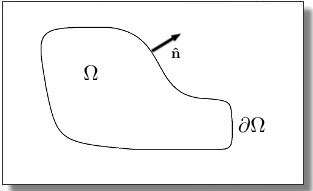
\includegraphics[width=0.475\textwidth]{geometry.jpg}
  \end{center}
  \caption{Geometry setup in \textsc{Ferret}.
%
$\Omega$ is completely bounded by surface $\partial \Omega$. $\hat{\textbf{n}}$ is an \emph{outward} facing surface normal.
%
The volume and the surface may exist as set of subdomains, $\Omega_k \subseteq \Omega_{k+1} \subseteq ... \subseteq \Omega$ and $\partial \Omega_k \subseteq \partial \Omega_{k+1} \subseteq ... \subseteq \partial \Omega$.
%
This block decomposition proves useful when defining the material properties of the problem.} %it should be noted that Moose will rename this to "subdomain" instead of block in the near future
\end{wrapfigure}
%
%
\begin{equation}\tag{3}
0 = \frac{\partial F}{\partial u_i} \Rightarrow \sigma_{ij,j} = \frac{\partial}{\partial x_j} C_{ijkl} \left(\varepsilon_{kl} - \varepsilon_{kl}^\mathrm{misfit} \right) = 0,
\end{equation}
%
the so-called stress-divergence equation \cite{Morton1975, BowerBook}.
%

%
\subsubsection{Surface elastic problem}
%
\paragraph{}In a elastic material, a surface tension can arise from a free surface, $\partial \Omega$, bounding the body, $\Omega$.
%
Here, this surface tension, with the Gurtin-Murdoch approach \cite{Morton1975},  is related to surface tensorial quantities by
%
\begin{equation}\tag{3.1}
\sigma_{\alpha \beta}^s = \tau^0 \delta_{\alpha \beta} + C_{\alpha \beta \delta \gamma}^s \varepsilon_{\delta \gamma}^s
\end{equation}
%
where $\alpha, \beta, \gamma, \delta = 1,2$ denote crystallographic directions along the surface.
%
$C_{\alpha \beta \delta \gamma}^s$ is the surface elastic tensor, and $\varepsilon_{\delta \gamma}^s$ is a surface elastic strain. The surface elastic tensor obeys the minor symmetries $C_{\alpha \beta \gamma \delta}^s = C_{\alpha \beta \delta \gamma }^s$ and $C_{\alpha \beta \delta \gamma}^s = C_{\beta \alpha \delta \gamma }^s$ and therefore has at most nine independent components.
%
The tension, $\tau^0$ is the intrinsic surface tension.
%
A surface free energy, $F_\mathrm{surface}$ can be introduced as,
%
\begin{equation}\tag{3}
F_\mathrm{surface} = \frac{1}{2} \int\limits_{\delta \Omega} d^2 \textbf{r} \,\,\, C_{\alpha \beta \delta \gamma }^s \varepsilon_{\alpha \beta}^s \varepsilon_{\delta \gamma}^s 
\end{equation}
%
with
%
\begin{equation}\tag{4}
 \varepsilon_{\alpha \beta}^s = \frac{1}{2} \left(\frac{\partial u_\alpha}{\partial x_\beta} + \frac{\partial u_\beta}{\partial x_\alpha} \right).
\end{equation}
%
The purely elastic free energy balance of the volume $\Omega$ bounded by $\delta \Omega$ with body forces $\textbf{b}$ and traction $\tau$ upon the surface, under an infinitesimal displacement field $\textbf{u}$, is
%
\begin{align}\tag{5}
 \frac{1}{2} \int\limits_\Omega C_{ijkl} \varepsilon_{ij} \varepsilon_{kl} \,\,d^3 \textbf{r} + \frac{1}{2} \int\limits_{\delta \Omega} \,\, C_{\alpha \beta \delta \gamma}^s \varepsilon_{\alpha \beta}^s \varepsilon_{\delta \gamma}^s\,\, d^2 \textbf{r} = \int\limits_\Omega \textbf{b} \cdot \textbf{u} \,\,\,d^3 \textbf{r} + \int\limits_{\partial \Omega} \tau \cdot \mathbf{\hat{n}} \,\,d^2 \textbf{r} - \int\limits_{\partial \Omega} \tau^0_{\alpha \beta} \varepsilon_{\alpha \beta}^s \,\,d^2 \textbf{r} \\ \nonumber
\end{align}
%
for some surface normal $\mathbf{\hat{n}}$.
%
Enforcing stationary under first-order variations \cite{BowerBook}, gives us three $(k = 1,2,3)$ weak form of the equations suitable for Galerkin finite element analysis, with test function $\psi_h$:
%
\begin{align}\tag{6}
 0 = \int\limits_\Omega C_{ijkl} \frac{\partial u_i}{\partial x_j} \frac{\partial \psi_h}{\partial x_l} d^3 \textbf{r} + \int\limits_{\partial \Omega} C_{ijkl}^s \left(\frac{\partial u_i}{\partial x_j} \frac{\partial \psi_h}{\partial x_k} \right)_s d^2 \textbf{r} - \int\limits_\Omega b_k \psi_h d^3 \textbf{r} - \int\limits_{\partial \Omega} \tau_k \psi_h d^2 \textbf{r} + \int\limits_{\partial \Omega} \left(\tau_{ij}^0 \frac{\partial \psi_h}{\partial x_j} \right)_s d^2 \textbf{r}.
\end{align}
%
The notation $\left( . \right)_s$ denotes the projection of the tensor onto the surface.
%
These quantities are constructed and each quadrature point on the finite element mesh surface by taking their bulk counterparts and using a local projection operator $\mathbf{\hat{\textbf{D}}} = \mathds{1} - \mathbf{\hat{n}}(\textbf{r}) \otimes \mathbf{\hat{n}} (\textbf{r})$ \cite{Yvonnet2012} such that 
%
\begin{align}\tag{7}
\sigma^s = \mathbf{\hat{\textbf{D}}} \sigma \mathbf{\hat{\textbf{D}}} \,\,\,\mathrm{and}\,\,\, \varepsilon^s = \mathbf{\hat{\textbf{D}}} \varepsilon \mathbf{\hat{\textbf{D}}}.
\end{align}
%
For application of this technique, see Influence of Elastic and Surface Strains on the Optical Properties of Semiconducting Core-Shell Nanoparticles,
John Mangeri, Olle Heinonen, Dmitry Karpeyev, and Serge Nakhmanson, Phys. Rev. Applied 4, 014001 -- \href{http://journals.aps.org/prapplied/abstract/10.1103/PhysRevApplied.4.014001}{Published}  7 July 2015. 
%

%
\subsection{Ferroelectric materials below $T_C$}
%

%
\paragraph{}A distinct feature of ferroelectric materials is their ability to form polar domains under certain conditions.
%
As the material is cooled down below the Curie temperature, its local polarization evolves towards thermodynamic equilibrium.
%
In the absence of an applied field (or some other ordering influence), the stationary state of the polarization distribution throughout the material is usually a complex equilibrium pattern\footnote[1]{Which is not the true global energy minimum of the system, but rather a local metastable energy minimum \cite{Hu1998}.} pattern, known as the \emph{domain structure}.
%
An important technical question, that was originally highlighted by Hu and Chen \cite{Hu1998, Li2001}, is how one can predict the equilibrium inhomogeneous ferroelectric microstructure --- or the `shape' of the polarization field $\mathbf{P}(\mathbf{r})$ --- while making no particular assumptions about its initial state?
%
Following the work of Su and Landis \cite{Su2007} and starting from the elementary second law of thermodynamics\footnote[2]{The second law states that the total entropy of an isolated system can only increase in time.
%
Mathematically, it can be written as
%
$$dS > dQ/T$$
%
for entropy $S$, temperature $T$, and heat $Q$.
%
Implicit within this statement is that the process is irreversible, which is the case of the domain structure formation as ferroic material is cooled below $T_C$.}, one can derive a time-dependent equation describing the evolution of $\mathbf{P}(\mathbf{r})$ that has the form of the celebrated Allen-Cahn equation \cite{Chan1977, LandauBook, Allen1979}.
%
%
\begin{align}\label{eq:time-dependent_landau_ginzburg_devonshire}
\frac{\partial P_i}{\partial t} = -\Gamma \frac{\delta }{\delta P_i}\Bigg(F\left[P_i\right] \Bigg)\,\,\mathrm{for} \,\,i = 1,2,3,
\end{align}
%
where the term in brackets is the variational derivative \footnote[3]{Variational derivative (sometimes called functional derivative) relates a change in a functional to a change in the function that functional depends on.
%
Let
%
$$J[f] = \int L[x,f,f'] dx,$$
%
where $J$ is a functional of $L$ that depends on $f = f(x)$, with $f'$ being the derivative of $f$ with respect to $x$. Then
%
$$\frac{\delta J}{\delta f} = \frac{\partial L}{\partial f} - \frac{d}{dx} \frac{\partial L}{\partial f'}.$$
%
This is also known as the Euler-Lagrange equation, if equated to zero \cite{GelfandBook}.
} with respect to $P_i$.
%
This equation is known as the time-dependent Landau-Ginzburg-Devonshire equation (TDLGD) and can be used to predict, with some general assumptions about initial conditions, the equilibrium polar domain structure within a ferroelectric system at a given temperature and elastic/electric boundary conditions.
%

%
The value of $\Gamma$ that has to be adopted for generic ferroelectric materials is still a subject of an extensive debate. Some researchers have suggested that $\Gamma$ can depend on the strength of the applied electric field during hysteretic switching \cite{Meng2015}.
%
Reasonable assumptions about $\Gamma$ for certain electric poling scenarios have produced good agreement with experimental results, such as the coercive field magnitudes and relaxation times of the polar field \cite{Fridkin2000, Hlinka2007}.
%
For most problems, the material coefficient is set to unity and as such, the system governing equations are solved in scaled time until a local minima has been found.
%
The total energy, $F$, can be written as an integral over a linear combination of energy densities,
%
$$F = \int\limits_\Omega d^3 \textbf{x} \Bigg[f_\mathrm{bulk} + \widetilde{f}_\mathrm{elastic} + f_\mathrm{elec} + f_\mathrm{grad} \Bigg].$$
%
In standard fashion, the bulk free energy density, $f_\mathrm{bulk}$ is expanded to sixth order,
%
$$f_\mathrm{bulk} = \alpha_{i} P_i + \beta_{ij} P_i P_j + \gamma_{ijk} P_i P_j P_k + \delta_{ijkl} P_i P_j P_k P_l  + \epsilon_{ijklm} P_i P_j P_k P_l P_m + \zeta_{ijklmn} P_i P_j P_k P_l P_m P_n.$$
%
The elastic energy density, 
%
$$\widetilde{f}_\mathrm{elastic} = \frac{1}{2} C_{ijkl} \left(\varepsilon_{ij} - \varepsilon_{ij}^0 \right) \left(\varepsilon_{kl} - \varepsilon_{kl}^0 \right) $$
%
contains the stress-free strain
%
$$\varepsilon_{kl}^0 = Q_{klmn} P_m P_n,$$
%
that arises due to the polarization for some electrostrictive coefficient tensor, $Q_{ijkl}$, of rank four. 
%
Note that this term can be decomposed into two terms (one of which explicitly contains the polarization field) in which we write $\widetilde{f}_\mathrm{elastic} = f_\mathrm{elastic}( \varepsilon_{ij}) + f_\mathrm{coupled}(\textbf{P}, \varepsilon_{ij})$.
%
The elastic displacement vectors (and their corresponding strain fields) should obey mechanical equilibrium (stress-divergence equation), namely,
%
\begin{align}\nonumber
\frac{\partial}{\partial x_i} \left[C_{ijkl} \left(\varepsilon_{ij} -  \varepsilon_{ij}^0 \right)\right] = 0
\end{align}

%
The electrostatic energy density term is written in the following fashion, 
%
\begin{align}\nonumber
f_\mathrm{electrostatic} &= - \frac{1}{2} E_k D_k\\ \nonumber
&= \frac{1}{2} \frac{\partial \Phi_\mathrm{int}}{\partial x_k} D_k\\ \nonumber
&= \frac{1}{2} \frac{\partial \Phi_\mathrm{int}}{\partial x_k} \left[- \epsilon_b \epsilon_0 \frac{\partial \Phi_\mathrm{int}}{\partial x_k}  + P_k\right]\\ \nonumber
\end{align}
%
using $E_k = - \partial \Phi_\mathrm{int} / \partial x_k$ and $D_k = \epsilon_b \epsilon_0 E_k + P_k$ with $\Phi_\mathrm{int}$ being the electrostatic potential generated by the Poisson equation\footnote[4]{The factor of $\frac{1}{2}$ in $f_\mathrm{electrostatic}$ being physically significant due to the adiabatic charging of the capacitor.},
%
$$\frac{\partial}{\partial x_j} \left( \epsilon_b \epsilon_0 \frac{\partial \Phi_\mathrm{int}}{\partial x_j}\right) = \frac{\partial P_k}{\partial x_k},$$
%
where $\rho_b = - \frac{\partial P_k}{\partial x_k}$ is the bound polarization charge density.
%
The parameter $\epsilon_b$ is the dielectric constant of the ferroelectric medium due to the core-electrons (sometimes noted as $\epsilon^\infty$ in DFT routines).
%
For the purposes of the perovskite-ferroelectrics, $\epsilon_b$ is about $5-10$ in units of vacuum permittivity. 
%
Externally to the ferroelectric medium, 
%
$$\frac{\partial}{\partial x_j} \left( \epsilon_{b,e} \epsilon_0 \frac{\partial \Phi_\mathrm{int}}{\partial x_j}\right) = 0$$
%
where the subscript $b,e$ denotes the dielectric constant of the external medium in units of $\epsilon_0$.
%
The energy density due to local gradients of the polarization, usually called the Ginzburg functional is, 
%
$$f_\mathrm{grad} = \frac{1}{2} G_{ijkl} \frac{\partial P_i}{\partial x_j} \frac{\partial P_k}{\partial x_l}.$$
%


%
\subsection{The case of the proper cubic-tetragonal phase transition}
%

%
\paragraph{}The coefficient tensors, $\alpha_{i}$, $\beta_{ij}$, $\gamma_{ijk}$, $\delta_{ijkl}$, $\epsilon_{ijklm}$, $\zeta_{ijklmn}$, $G_{ijkl}$, and $Q_{mnkl}$,  and $C_{ijkl}$ are material dependent, obey symmetries of the lattice, and in general can be dependent at temperature, $T$.
%
Symmetrizing the energy density terms for the case of a cubic parent phase, one writes
%
\begin{align}\nonumber
f_\mathrm{bulk} &= \alpha_1 \left(P_x^2 + P_y^2 + P_z^2 \right) + \alpha_{11} \left(P_x^4 + P_y^4 + P_z^4 \right) + \alpha_{12} \left(P_x^2 P_y^2 + P_y^2 P_z^2 + P_x^2 P_z^2 \right) \\ \nonumber
&+ \alpha_{111} \left(P_x^6 + P_y^6 + P_z^6 \right) + \alpha_{112} \left[P_x^4 \left(P_y^2 + P_z^2 \right) + P_y^4 \left(P_x^2 + P_z^2 \right) + P_z^4 \left(P_x^2 + P_y^2 \right) \right] + \alpha_{123} \left(P_x^2 P_y^2 P_z^2 \right), \\ \nonumber
\end{align}
%
and
%
\begin{align}\nonumber
f_\mathrm{grad} &= \frac{1}{2} G_{11} \left[\left(\frac{\partial P_x}{\partial x} \right)^2 \hspace{-1pt}+\hspace{-1pt} \left(\frac{\partial P_y}{\partial y}\right)^2 \hspace{-1pt}+\hspace{-1pt}\left( \frac{\partial P_z}{\partial z} \right)^2\right] \\ \nonumber
&+ G_{12} \left[\frac{\partial P_x}{\partial x}\frac{\partial P_y}{\partial y}\hspace{-2pt} +\hspace{-1pt} \frac{\partial P_y}{\partial y} \frac{\partial P_z}{\partial z}\hspace{-2pt} +\hspace{-1pt} \frac{\partial P_x}{\partial x} \frac{\partial P_z}{\partial z} \right] \\ \nonumber
&+ \hspace{-2pt} \frac{1}{2} G_{44}  \hspace{-2pt}\left[\left(\frac{\partial P_x}{\partial y} \hspace{-1pt}+ \hspace{-1pt} \frac{\partial P_y}{\partial x} \right)^2 \hspace{-6pt}+\hspace{-2pt} \left(\frac{\partial P_y}{\partial z} \hspace{-1pt}+ \hspace{-1pt}\frac{\partial P_z}{\partial y} \right)^2 \hspace{-6pt}+\hspace{-2pt} \left(\frac{\partial P_x}{\partial z} \hspace{-1pt}+\hspace{-1pt} \frac{\partial P_z}{\partial x} \right)^2  \hspace{-0.5pt}\right] \\ \nonumber
&+ \hspace{-2pt}\frac{1}{2} G'_{44} \hspace{-2pt}\left[\left(\frac{\partial P_x}{\partial x_2} \hspace{-1pt}- \hspace{-1pt}\frac{\partial P_y}{\partial x} \right)^2 \hspace{-6pt} + \hspace{-2pt} \left(\frac{\partial P_y}{\partial z}\hspace{-1pt} - \hspace{-1pt}\frac{\partial P_z}{\partial y} \right)^2 \hspace{-6pt}+  \hspace{-2pt}\left(\frac{\partial P_x}{\partial z}\hspace{-1pt} - \hspace{-1pt}\frac{\partial P_z}{\partial x} \right)^2 \hspace{-0.5pt} \right].
\end{align}
%
with sign and factor of 2 convention from Ref. \cite{Li2001, Hlinka2006}. By forcing the $f_\mathrm{coupled}$ term to respect the $O_h$ point group symmetry of the parent phase, one can show
%
\begin{align}\nonumber
2 f_\mathrm{coupled} &= \frac{\partial u_x}{\partial x} \left(C_{11} Q_{11} + 2 C_{12} Q_{12} \right) P_x^2 + \frac{\partial u_x}{\partial x} \left[C_{11} Q_{12} + C_{12} \left(Q_{11} + Q_{12} \right)\right] P_y^2 \\ \nonumber
&+ \frac{\partial u_x}{\partial x} \left[C_{11} Q_{12} + C_{12} \left(Q_{11} + Q_{12} \right)\right] P_z^2 + 2 C_{44} \frac{\partial u_x}{\partial y} Q_{44} P_x P_y  + 2 C_{44} \frac{\partial u_x}{\partial z} Q_{44} P_x P_z\\ \nonumber
&+ 2 C_{44} \frac{\partial u_y}{\partial x} Q_{44} P_x P_y + \frac{\partial u_y}{\partial y} \left[C_{11} Q_{12} + C_{12} \left(Q_{11} + Q_{12} \right)\right] P_x^2 + \frac{\partial u_y}{\partial y} \left(C_{11} Q_{11} + 2 C_{12} Q_{12}\right) P_y^2 \\ \nonumber
&+ \frac{\partial u_y}{\partial y} \left[C_{11} Q_{12} + C_{12} \left(Q_{11} + Q_{12} \right)\right]  P_z^2 + 2 C_{44} \frac{\partial u_y}{\partial z} Q_{44} P_y P_z + 2 C_{44} \frac{\partial u_z}{\partial x} Q_{44} P_x P_z \\ \nonumber
&+ 2 C_{44} \frac{\partial u_z}{\partial y} Q_{44} P_y P_z + \frac{\partial u_z}{\partial z} \left[C_{11} Q_{12} + C_{12} \left(Q_{11} + Q_{12} \right)\right] P_x^2 \\ \nonumber
&+ \frac{\partial u_z}{\partial z} \left[C_{11} Q_{12} + C_{12} \left(Q_{11} + Q_{12} \right)\right] P_y^2 + \frac{\partial u_z}{\partial z} \left(C_{11} Q_{11} + 2 C_{12} Q_{12} \right) P_z^2
\end{align}
%
where $\textbf{u} = \langle u_x, u_y, u_z \rangle$ is the elastic displacement vector.
%

%

%
\section{Comments on the natural boundary condition of the paraelectric-ferroelectric interface}
%

%
\textsc{Ferret} uses a finite element approach which utilizes a weak form variation of the partial differential equations to be solved.
%
The potential field, $\Phi = \Phi(\textbf{x})$, in some volume $V$ due to a charge distribution $\rho$, satisfies the following PDE,
%
\begin{align}\label{eq:poisson_problem_1}
\frac{\partial}{\partial x_i} \left(\epsilon_b(\textbf{x}) \frac{\partial \Phi(\textbf{x})}{\partial x_i}\right) = \frac{\partial P_j(\textbf{x})}{\partial x_j},
\end{align}
%
where the charge distribution is solely comprised of bound charges $\rho_b = -\nabla \cdot \textbf{P}$, with polarization field $\textbf{P}$ that could be zero, fixed, or vary in space.
%
%The origin (and definitions) of these variables are defined in a previous chapter.
%
We again employ Einstein's summation convention for repeated indices. 
%
The dielectric constant, $\epsilon_b(\textbf{x})$, is assumed to be a scalar function of space (no anisotropy).
%
%For now, $\textbf{P}$ can be considered as a fixed quantity (that could vary in space), but later in this Chapter, it will be a \emph{variable} to be solved for (in the same manner as $\Phi$) within the variational approach when coupled to the TDLGD equations. %%%%I don't understand what you're saying here about P.  Right now, it's not a variable?
%%%%This whole 2nd half of the paragraph doesn't flow very well, it feels like things kind of jump around.
%

%
Eq.~(\ref{eq:poisson_problem_1}) is a boundary value problem that is only solvable when the value of $\Phi$ is defined upon some boundary. 
%
This PDE is a so-called \emph{strong} problem statement that must be converted into a \emph{weak} form.
%
This is done as follows by constructing a \emph{residual} statement of this boundary-value problem,
%
\begin{align}\label{eq:poisson_problem_2}
r(\textbf{x}) = \frac{\partial}{\partial x_i} \left(\epsilon_b(\textbf{x}) \frac{\partial \Phi(\textbf{x})}{\partial x_i}\right) - \frac{\partial P_j(\textbf{x})}{\partial x_j} = 0.
\end{align}
%
We ``test'' this residual over arbitrary subregions by multiplying it by a sufficiently smooth test function $v(\textbf{x})$.
%
The residual is then integrated over the domain $V$,\footnote[5]{The L2 space of $v$ must be smooth enough to be square integrable over the volume, or $\int_V \left\{[\nabla v(\textbf{x})]^2 + v(\textbf{x})^2 \right\} dV < \infty$.
%
We call these class of functions $H^1(V)$ where the $1$ denotes that the first derivative is square integrable.} i.e.,
%
\begin{align}\label{eq:poisson_problem_3}
\mathscr{R} = \iiint\limits_V d^3 \textbf{x} \, v(\textbf{x})\,\frac{\partial}{\partial x_i} \left(\epsilon_b(\textbf{x}) \frac{\partial \Phi(\textbf{x})}{\partial x_i}\right) - \iiint\limits_V d^3 \textbf{x} \, v(\textbf{x})\, \frac{\partial P_j(\textbf{x})}{\partial x_j} = 0.
\end{align}
%
Integration by parts allows us to obtain an expression with terms only containing first derivatives of $\Phi$ and $\textbf{P}$, 
%
\begin{align}\label{eq:poisson_problem_4}
\mathscr{R} = \iiint\limits_V d^3 \textbf{x} \, \frac{\partial v(\textbf{x})}{\partial x_i} \, \epsilon_b(\textbf{x}) \, \frac{\partial \Phi(\textbf{x})}{\partial x_i} - \iiint\limits_V d^3 \textbf{x} \, v(\textbf{x})\, \frac{\partial P_j(\textbf{x})}{\partial x_j} - \oiint\limits_S d^2 \textbf{x} \, \left[\epsilon_b(\textbf{x}) \frac{\partial \Phi}{\partial x_i} \hat{n}_i v(\textbf{x})\right] = 0,
\end{align}
%
where we have transformed the second volume integral (over $\Phi$) to a surface integral (with outward-facing surface normal $\hat{\textbf{n}}$) by using the divergence theorem. 
%
The term involving $\textbf{P}$ can also be processed in the same fashion, %%%Why did you do this, if P already is only first derivative - to remove the derivative entirely and put it onto the test function?  This is a subtle point. -a
% I'll leave this comment here. -j
%
\begin{align}\label{eq:poisson_problem_5}
\mathscr{R} &= \iiint\limits_V d^3 \textbf{x} \, \frac{\partial v(\textbf{x})}{\partial x_i} \, \epsilon_b(\textbf{x}) \, \frac{\partial \Phi(\textbf{x})}{\partial x_i} - \iiint\limits_V d^3 \textbf{x} \, \frac{\partial v(\textbf{x})}{\partial x_j}\, P_j(\textbf{x}) \\ \nonumber
&- \oiint\limits_S d^2 \textbf{x} \, \left[\epsilon_b(\textbf{x}) \frac{\partial \Phi}{\partial x_i} \hat{n}_i v(\textbf{x})\right] + \oiint\limits_S d^2 \textbf{x} \, \left[ P_k \hat{n}_k v(\textbf{x})\right] \\ \nonumber
&= 0,
\end{align}

%
%If $\textbf{P} = 0$ and $V = V_1 \cup V_2$ where there are discontinuous constants $\epsilon_{b,1} \neq \epsilon_{b,2}$ in $V_1$ and $V_2$ respectively, then we get the natural boundary conditions \cite{CareyBook} ($\nabla \Phi \cdot \hat{n} = 0$) that are required by the electrostatics (these are tangential electric fields need to be continuous and the perpendicular component of the electric \emph{displacement} $\textbf{D}$ must be discontinuous \cite{JacksonBook}).
%
%The finite element solution of such a problem [Eq. (\ref{eq:poisson_problem_5}) without $\textbf{P}$ and block restricted $\epsilon_b(\textbf{x})$ is simply Laplace's problem] give \emph{exact} analytic results in \textsc{MOOSE}.
%
%Comparison between numerical and analytical results for Laplace's and Poisson's problems are discussed later in this Chapter.
%

%
Eq.~(\ref{eq:poisson_problem_5}) contains both volume and boundary terms.
%
As mentioned before, the boundary-value problem requires well-defined boundary conditions in order to be solved.
%
Now, note that if
%
\begin{align}\label{eq:neumann_bc}
\frac{\partial A(\textbf{x})}{\partial x_k} \hat{n}_k = g (\textbf{x})\,\,\mathrm{on}\,\, S_1 \subseteq S,
\end{align}
%
where $g(\textbf{x})$ is some nonzero function, $A(\textbf{x})$ is the variable we are solving for, and $S_1 \cup S_2 = S$ is the boundary where this is satisfied then Eq.~(\ref{eq:neumann_bc}) represents a \emph{Neumann boundary condition}.  
%
If such a boundary condition is present for $\Phi$ on $S_1$ then  Eq.~(\ref{eq:poisson_problem_5}) becomes,
%
\begin{align}\label{eq:poisson_problem_5_BC}
\mathscr{R} &= \iiint\limits_V d^3 \textbf{x} \, \frac{\partial v(\textbf{x})}{\partial x_i} \, \epsilon_b(\textbf{x}) \, \frac{\partial \Phi(\textbf{x})}{\partial x_i} - \iiint\limits_V d^3 \textbf{x} \, \frac{\partial v(\textbf{x})}{\partial x_j}\, P_j(\textbf{x}) \\ \nonumber
&- \oiint\limits_{S_2} d^2 \textbf{x} \, \left[\epsilon_b(\textbf{x}) \frac{\partial \Phi}{\partial x_i} \hat{n}_i v(\textbf{x})\right] + \oiint\limits_{S_2} d^2 \textbf{x} \, \left[ P_k \hat{n}_k v(\textbf{x})\right] \\ \nonumber
&- \oiint\limits_{S_1} d^2 \textbf{x} \, \left[\epsilon_b(\textbf{x}) \,g(\textbf{x})\, v(\textbf{x})\right] \\ \nonumber
&= 0,
\end{align}
%
where the integration over the surface has been split into regions $S_1$ and $S_2$ to emphasize the application of the Neumann boundary condition.
%
The ``natural'' boundary condition, applied to region $S_2$ where the value of $\frac{\partial A(\textbf{x})}{\partial x_k} \hat{n}_k $ is unspecified but still contributes to the residual value \emph{to be minimized}, is a special case of the Neumann boundary condition.
%
In that case, Eq.~(\ref{eq:poisson_problem_5}) would be unchanged.
%
For the boundary value problem, there is another type of boundary condition that could be specified (Dirichlet) which involves constraining the value of the variables at the nodes - removing the degrees of freedom of the problem. 
%

%
%\subsection{Some brief comments on the finite element approach}
%%
%
%%
%At this stage, the finite element approximation to both $v, \Phi, S$ and $V$ is required.
%%
%The volume $V$ and surface $S$ are discretized as described earlier, such that $V \approx V_h$ and $S \approx S_h$, with the coordinates of each $j^\mathrm{th}$ node given by $(x_j, y_j, z_j )$ in Cartesian coordinates\footnote[6]{To be sufficiently general, there is nothing that requires that we work in Cartesian coordinates. 
%%
%For example, MOOSE can perform simulations with a range of coordinate systems (and residual construction can be done with coordinate-free operators).} for $j = \{1, 2, ... N \}$.
%%
%The test function $v$ can be expanded as a linear sum of shape (basis) functions [$\phi_j = \phi_j(\textbf{x})$] such that 
%%
%\begin{align}\label{eq:shape}
%v_h(\textbf{x}) = \sum\limits_{j = 1}^N v_j \phi_j(\textbf{x})
%\end{align}
%%
%where $N$ is the number of nodes in the mesh and $v_j$ are \emph{unknown}\footnote[7]{This is an important detail here.
%%
%The unidentified values of the expansion coefficients are precisely what we solve for in the FEM.} expansion coefficients.
%%
%Many different choices for $\phi_j(\textbf{x})$ exist.
%%
%Shape or basis functions could be piecewise-linear, quadratic, cubic, or even higher order \cite{CareyBook}.
%%
%The optimum choice of $\phi_j(\textbf{x})$ typically depends on a specific that needs to be solved,
%including the desired solution accuracy and computational efficiency.
%%
%%
%In particular, the piecewise linear (Lagrange) $\phi_i$ on some (unstructured or structured) one-dimensional mesh,
%%
%\begin{align}\label{eq:piecewise_linear}
%\phi_i (x) = \begin{cases}
%    \frac{x - x_j}{x_i - x_j}, & \mathrm{if} \,\,x_j < x \leq x_i \\
%    \frac{x_j - x}{x_j - x_i}, & \mathrm{if} \,\,x_i < x \leq x_j, \\
%  \end{cases}
%\end{align}
%%
%Therefore, the following relationship is established,
%%
%\begin{align}\label{eq:node_basis}
%\phi_i (\textbf{x}_j) = \delta_{ij},
%\end{align}
%%
%which forces the value of the function to unity at the node.
%%
%%The value of the basis function not at the node can be anything but usually it is chosen to decay away.
%%
%For a node located at $\textbf{x}_i$ then Eq.~(\ref{eq:piecewise_linear}) gives $v_h(\textbf{x}_i) = v_i$ (equal to the $i^\mathrm{th}$ coefficient). %%%I think this is strictly true only for linear Lagrange.  The basis (shape) functions overlap in space...  -a
%% I'll check this then -j
%%
%%An example of Eq.~(\ref{eq:piecewise_linear}) on a uniform (structured) one-dimensional mesh is shown in Fig.~\ref{fig} \textbf{to be made}.
%%
%The variable of interest $\Phi_h(\textbf{x})$ is also expanded in terms of the same basis functions $\phi_j$ which gives
%%
%\begin{align}\label{eq:variable_potential}
%\Phi_h (\textbf{x}) = \sum\limits_{j= 1}^N \Phi_j \phi_j(\textbf{x}),
%\end{align}
%%
%for some unknown coefficients $\Phi_j$\footnote[8]{The quantity $\textbf{P}$ for purposes of this discussion can be considered as a constant (nonzero or zero) as mentioned above.}.
%%
%Introducing Eq.~(\ref{eq:shape}) and Eq.~(\ref{eq:variable_potential}) into the above Eq.~(\ref{eq:poisson_problem_5}) that are integrated over $V_h$ enclosed by $S_h$ gives, 
%%
%\begin{align}\label{eq:poisson_problem_6}
%\mathscr{R} &= \sum\limits_{r=1}^N \sum\limits_{s=1}^N \left(\iiint\limits_{V_h} d^3 \textbf{x} \, \frac{\partial \left[v_r \phi_r(\textbf{x})\right]}{\partial x_i} \, \epsilon_b(\textbf{x}) \, \frac{\partial \left[\Phi_s \phi_s(\textbf{x})\right]}{\partial x_i} \right)- \sum\limits_{r=1}^N\left(\iiint\limits_{V_h} d^3 \textbf{x} \, \frac{\partial \left(v_r \phi_r(\textbf{x})\right)}{\partial x_j}\, P_j(\textbf{x}) \right)\\ \nonumber
%&-\sum\limits_{r=1}^N \sum\limits_{s=1}^N \left( \oiint\limits_{S_h} d^2 \textbf{x} \, \left[\epsilon_b(\textbf{x}) \frac{\partial \left[\Phi_s \phi_s(\textbf{x})\right]}{\partial x_i} \hat{n}_i v_r \phi_r(\textbf{x})\right]\right) + \sum\limits_{r=1}^N\left(\oiint\limits_{S_h} d^2 \textbf{x} \, \left[  P_j(\textbf{x}) \hat{n}_j v_r \phi_r(\textbf{x})\right] \right) = 0,
%\end{align}
%%
%where now we searching for an approximate solution to Eq.~(\ref{eq:poisson_problem_5}).
%%
%The coefficients $v_r, \Phi_s$ do not depend on space, so they can be pulled out of the integrals, giving,
%%
%\begin{align}\label{eq:poisson_problem_7}
%\mathscr{R} &= \sum\limits_{r=1}^N \sum\limits_{s=1}^N \left(v_r \Phi_s \iiint\limits_{V_h} d^3 \textbf{x} \, \frac{\partial \phi_r(\textbf{x})}{\partial x_i} \, \epsilon_b(\textbf{x}) \, \frac{\partial \phi_s(\textbf{x})}{\partial x_i} \right) - \sum\limits_{r=1}^N  v_r \left( \iiint\limits_{V_h} d^3 \textbf{x} \, \frac{\partial \phi_r(\textbf{x})}{\partial x_j}\, P_j(\textbf{x}) \right)\\ \nonumber
%&-\sum\limits_{r=1}^N \sum\limits_{s=1}^N \left( v_r \Phi_s \oiint\limits_{S_h} d^2 \textbf{x} \, \left[\epsilon_b(\textbf{x}) \frac{\partial \phi_s(\textbf{x})}{\partial x_i} \hat{n}_i \phi_r(\textbf{x})\right]\right) + \sum\limits_{r=1}^N v_r \left(\oiint\limits_{S_h} d^2 \textbf{x} \, \left[  P_j(\textbf{x}) \hat{n}_j \phi_r(\textbf{x})\right] \right) = 0.
%\end{align}
%%
%This equation can be rearranged, 
%%
%\begin{align}\label{eq:poisson_problem_8linear}
%\sum\limits_{r=1}^N v_r \left(\sum\limits_{s=1}^N K_{rs} \Phi_s - F_r \right) = 0.
%\end{align}
%%
%where
%%
%\begin{align}\label{eq:poisson_problem_constant_P_stiffness}
%K_{rs} = \iiint\limits_{V_h} d^3 \textbf{x} \, \frac{\partial \phi_r(\textbf{x})}{\partial x_i} \, \epsilon_b(\textbf{x}) \, \frac{\partial \phi_s(\textbf{x})}{\partial x_i} -  \oiint\limits_{S_h} d^2 \textbf{x} \, \left[\epsilon_b(\textbf{x}) \frac{\partial \phi_s(\textbf{x})}{\partial x_i} \hat{n}_i \phi_r(\textbf{x})\right]
%\end{align}
%%
%and
%%
%\begin{align}\label{eq:poisson_problem_constant_P_load}
%F_r = \iiint\limits_{V_h} d^3 \textbf{x} \, \frac{\partial \phi_r(\textbf{x})}{\partial x_j}\, P_j(\textbf{x}) - \oiint\limits_{S_h} d^2 \textbf{x} \, \left[  P_j(\textbf{x}) \hat{n}_j \phi_r(\textbf{x})\right],
%\end{align}
%%
%are the \emph{stiffness} matrix and \emph{load} vectors, respectively.
%%
%The problem defined in Eq. (\ref{eq:poisson_problem_8linear}) contains a linear system of equations,
%%
%\begin{align}\label{eq:poisson_problem_linear_system}
%\sum\limits_{s=1}^N K_{rs} \Phi_s - F_r = 0.
%\end{align}
%%
%to be solved for $N$ values of $\Phi_s$ (the unknown degrees of freedom of the problem). 
%%
%If $P_j(\textbf{x}) = 0$ then we have Laplace's problem (a homogeneous system of linear equations).
%%
%However, if $P_j(\textbf{x}) \neq 0$ then we have Poisson's problem and the polarization values will be contained within the load vector $F_r$\footnote[9]{Elementary linear algebra states that the solution of such an equation is $\Phi_r = \sum_{s=1}^N (K^{-1})_{sr} F_r$.
%%
%Of course if $F_r = 0 \, \forall \, r$, then Eq. (\ref{eq:poisson_problem_linear_system}) is a homogeneous system of linear equations with a trivial solution.
%%
%If a non-trivial solution exists, it can be found by singular value decomposition or other linear algebra approaches.
%}.
%%
%
%%
%Finally, at this point, the Dirichlet boundary condition can be set within the linear system residual statement, Eq. (\ref{eq:poisson_problem_linear_system}).
%%
%The values of the $\Phi$ vector are set as $\Phi_{s'} = \widetilde{\Phi}_{s'}$ for every node $s'$ that lives on some boundary $S_{h,1} \in S_h$. 
%%
%For example, in matrix form, this would be
%%
%\begin{align}\label{eq:dirichlet_bc}
%\Phi_s = \begin{pmatrix}
%    \Phi_{1}     \\
%    \Phi_{2}     \\
%    \Phi_{3}     \\
%    \vdots \\
%    \Phi_{N}      
%\end{pmatrix} \to \Phi_s = \begin{pmatrix}
%    \Phi_{1}       \\
%    \widetilde{\Phi}_{2} \\
%    \widetilde{\Phi}_{3} \\
%    \vdots   \\
%    \Phi_{N}      
%\end{pmatrix},
%\end{align}
%%
%where nodes $s' = 2$ and $s' = 3$ live on the boundary sideset of $S_{h,1}$ and have Dirichlet boundary conditions.
%%
%This means that the Dirichlet data for $\Phi_{s'} = \widetilde{\Phi}_{s'}$ reduces the number of degrees of freedom of the problem. 
%
%\textbf{It should be noted that MOOSE does not specifically use this FEM approach.}

%----------------------------------------------------------------------------------------
%	BIBLIOGRAPHY
%----------------------------------------------------------------------------------------
\begin{thebibliography}{1}
%\small{

\bibitem{Morton1975}
E.~Morton, G.~Gurtin, and A.~I.~Murdoch, 
%\newblock{A continuum theory of elastic material surfaces}
\newblock {\em Arch. Ration. Mech. Anal.} \textbf{57}, 291 (1975).

\bibitem{BowerBook}
A.~F.~Bower,
%\newblock {Applied Mechanics of Solids}.
\newblock \emph{Applied Mechanics of Solids.} CRC Press Inc. (2009).

\bibitem{NyeBook}
J.~F.~Nye,
%\newblock {Physical Properties of Crystals}.
\newblock \emph{Physical Properties of Crystals.} Oxford University Press Inc. (1985).

\bibitem{Yvonnet2012}
J.~Yvonnet, A.~Mitrushchenkov, G.~Chambaud, Q.-C.~He, and S.-T.~Gu, 
%\newblock{Characterization of surface and nonlinearelasticity in wurtzite ZnO nanowires,}
\newblock {\em J. Appl. Phys} \textbf{111}, 124305 (2012).

\bibitem{LinesBook}
M.~E.~Lines, and A.~M.~Glass 
%\newblock{Princples and Applications of Ferroelectrics and Related Materials}
\newblock {\em Princples and Applications of Ferroelectrics and Related Materials} (Clarendon, Oxford, 1977).

\bibitem{RabeBook}
K.~M.~Rabe, C.~H.~Ahn, and J.-M.~Triscone
%\newblock {Physics of Ferroelectrics: A Modern Perspective}
\newblock {\em Physics of Ferroelectrics: A Modern Perspective} (Springer-Verlag, Berlin, 2007),

\bibitem{WootenBook}
M.~El-Batanouny, and F.~Wooten
%\newblock {Symmetry in Condensed Matter Physics: A Computational Approach}
\newblock {\em Symmetry in Condensed Matter Physics: A Computational Approach} (Cambridge, 2008),

\bibitem{FerretLink}
Link to Ferret code-repository: https://bitbucket.org/mesoscience/ferret

\bibitem{Gaston2009}
D.~Gaston, C.~Newman, G.~Hansen, D.~Lebrun-Grandi{\'{e}},
%\newblock {MOOSE: A parallel computational framework for coupled systems of
%  nonlinear equations}.
\newblock {\em Nucl.~Eng.~Design} \textbf{239}, 1768 (2009).

\bibitem{Kirk2006}
B.~S.~Kirk, J.~W.~Peterson, R.~H.~Stogner, and G.~F.~Carey,
%\newblock {libMesh: A C++ Library for Parallel Adaptive Mesh Refinement/Coarsening Simulations}.
\newblock {\em Eng.~with~Comp.} \textbf{22}(3-4), 237-254 (2006).

\bibitem{Su2007}
Y.~Su, and C.~M.~Landis,
%\newblock {Continuum thermodynamics of ferroelectric domain evolution: Theory, finite element implementation, and application to domain wall pinning}.
\newblock {\em J.~Mech.~Comp.~Phys.~Solids} \textbf{55}, 280-305 (2007).

\bibitem{Tonks2012}
M.~Tonks, D.~Gaston, P.~C.~Millet, D.~Anders, and P.~Talbot,
%\newblock {An object-oriented finite element framework for multiphysics phase field simulations}.
\newblock {\em Comp.~Mat.~Sci.} \textbf{51}, 20-29 (2012).

\bibitem{Dawber2005}   
M.~Dawber, K.~M.~Rabe, and J.~F.~Scott,
%Physics of thin-film ferroelectric oxides
\newblock {\em Rev.~Mod.~Phys.} \textbf{77}, (2005).

\bibitem{Nelson2011}
C.~T.~Nelson, P.~Gao, J.~R.~Jokisaari, C.~Heikes, C.~Adamo, A.~Melville, S.-H.~Baek, C.~M.~Folkman, B.~Winchester, Y.~Gu, Y.~Liu, K.~Zhang, 
E.~Wang, J.~Li, L.-Q.~Chen, C.-B.~Eom, D.~G.~Schlom, and X.~Pan,
%Domain Dynamics During Ferroelectric Switching
\newblock {\em Science} \textbf{334}, 968--971 (2011).

\bibitem{Baroni2001}
S.~Baroni, S.~Gironcoli, and A.~D.~Corso,
%\newblock {Phonons and related crystal properties from density-functional perturbation theory}.
\newblock \emph{Rev.~Mod.~Phys.} \textbf{73} (2001).

\bibitem{Eliseev2015}
E.~A.~Eliseev, S.~V.~Kalinin, and A.~N.~Morozovska,
%\newblock {Finite size effects in ferroelectric-semiconductor thin films under open-circuit electric boundary conditions}.
\newblock \emph{J.~Appl.~Phys.} \textbf{117}, 034102 (2015).

\bibitem{Hu1998}
H.~Hu, and L.-Q. Chen,
%\newblock {}.
\newblock \emph{J. Am. Ceram. Soc.} \textbf{81} [3] 492-500 (1998).

\bibitem{Li2001}
Y.~L.~Li, S.~Y.~Hu, Z.~K.~Liu, and L.-Q.~Chen,
%\newblock {Phase-field model of domain structures in ferroelectric thin films}.
\newblock \emph{Appl.~Phys.~Lett.} \textbf{78} 492--500 (2001).

\bibitem{Meng2015}
Q.~Meng, M.-G.~Han, J.~Tao, G.~Xu, D.~O.~Welch, and Y.~Zhu
%\newblock {}.
\newblock \emph{Phys.~Rev. B} \textbf{91} 054104 (2015).

\bibitem{Cao2008}
W.~Cao,
%\newblock {Constructing Landau-Ginzburg-Devonshire Type Models for Ferroelectric Systems based on Symmetry}.
\newblock \emph{Ferroelectrics.} 375:28-39 (2008).

\bibitem{Chan1977}
S.-K. Chan,
%\newblock {}.
\newblock \emph{J. Chem. Phys.} \textbf{67}, 5755-5762, (1977)

\bibitem{LandauBook}
L. D.~Landau, and I. M.~Khalatnikov
%\newblock {On the  theory  of  superconductivity}.
\newblock \emph{Collected Papers  of L.D.  Landau, (ed.  D. Ter  Haar), Pergamon,  Oxford} (1965)

\bibitem{Allen1979}
S.-K. Allen, and J. W. Cahn,
%\newblock {}.
\newblock \emph{Ada. Metall.} \textbf{27}, 1085-1095, (1979)


\bibitem{Fridkin2000}
V. M.~Fridkin, and S. Ducharme,
%\newblock {}.
\newblock \emph{Phys. Solid State} \textbf{43} 7, 1320-1324 (2001).

\bibitem{Hlinka2007}
J. ~Hlinka,
%\newblock {Mobility of ferroelastic domain walls in barium titanate}.
\newblock \emph{Ferroelectrics} \textbf{349} 499-544 (2007).


\bibitem{Hlinka2006}
J. ~Hlinka, and P. ~Marton
%\newblock {}.
\newblock \emph{Phys. Rev. B.} \textbf{74} 104014 (2006).

\bibitem{Pertsev1998}
N.~A.~Pertsev, A.~G.~Zembilgotov, and A.~K.~Tagantsev
%\newblock {Effect of Mechanical Boundary Conditions on Phase Diagrams of Epitaxial Ferroelectric Thin Films}.
\newblock \emph{Phys. Rev. Lett.} \textbf{80} 9 (1998).

\bibitem{Yin2010}
W.-J.~Yin, S.~Chen, J.-H, Yang, X.-G.~Gong, Y.~Yan, and S.-H.~Wei
%\newblock {Effective band gap narrowing of anatase TiO2 by strain along a soft crystal direction}.
\newblock \emph{Appl. Phys. Lett.} \textbf{96} 221901 (2010).

%\bibitem{Wagner2013}
%M.~R.~Wagner, G.~Callsen, J.~S.~Reparaz, R.~Kirste, A.~Hoffmann, A.~V.~Rodina, A.~Schleife, F.~Bechstedt, and M.~R.~Phillips
%%\newblock {Effects of strain on the valence band structure and exciton-polariton energies in ZnO}.
%\newblock \emph{Phys. Rev. B.} \textbf{88} 235210 (2013).

\bibitem{Wang2003}
B.~Wang, R.~Xia, H.~Fan, C.~H.~Woo,
%\newblock {Dynamic process of domain switching in ferroelectric films}.
\newblock \emph{J. Appl. Phys.} \textbf{94} 5 (2003).

\bibitem{Wang2011}
Y.-L.~Wang, X.-Y.~Wang, L.-Z.~Chu, Z.-C.~Deng, X.-C.~Ding, W.-H.~Liang, P.-C.~Zhang, L.~Liu, B.-T.~Liu, and G.-S.~Fu,
%\newblock {Simulation of the initial polarization curves and hyteresis loops for ferroelectric films by an extensive time-dependent Ginzburg-Landau model}.
\newblock \emph{J. Mater. Sci.} \textbf{46}:2695-2699 5 (2011).

\end{thebibliography}


%----------------------------------------------------------------------------------------

\end{document}